\documentclass{beamer}
\graphicspath{ {./images/} }

\mode<presentation> {
  \definecolor{frameheadforeground}{RGB}{169,33,62}
  \definecolor{frameheadbackground}{RGB}{255,255,255}

  \usetheme{Warsaw}
  %\setbeamercovered{transparent}
}

\setbeamercolor{structure}{fg=frameheadforeground,bg=frameheadbackground}

\usepackage[utf8]{inputenc}
\usepackage[MeX]{polski}

\begin{document}

\begin{frame}
\title[Tytuł]{Analiza wielowymiarowa}
\subtitle{Środowisko Pracy}
\author{Maciej Nasinski, Paweł Strawiński}
\institute{Uniwersytet Warszawski}
\date{Zajęcia 1 \\ 7 października 2021}
\titlepage
\end{frame}

\section{Środowisko}

\begin{frame}{Narzędzia}
  \begin{itemize}
  \item STATA 17 \url{https://www.wne.uw.edu.pl/pl/wydzial/pracownia-informatyczna/}
  \item anaconda (e.g. python packages i jupyter/jupyerlab) \url{https://www.anaconda.com/products/individual}
  \item git clone \url{https://github.com/Polkas/AW2021} albo sciągniecie i rozpakowanie
  \item Uzupełnienie AW2021/spec.yaml w tym otrzymanym hasłem od prowadzących
  \end{itemize}
\end{frame}

\begin{frame}{Odtworzenie Środowiska Pracy - Reprodukowalność}
  \begin{itemize}
  \item \texttt{terminal (zsh lub bash) oraz conda.}
  \item Anaconda Navigator - GUI.
  \end{itemize}
\end{frame}

\begin{frame}{Komputery prywatne - terminal}
  \begin{itemize}
  \item \texttt{conda create --yes --name py38\_aw\_wne python=3.8} 
  \item \texttt{conda activate py38\_aw\_wne}
  \item \texttt{pip3 install -r requirements.txt}
  \item \texttt{?OPCJONALNIE conda install SYSTEM\_SPECYFICZNE\_JAK\_PYWIN32}
  \item \texttt{jupyter lab}
  \end{itemize}
\end{frame}

\begin{frame}{WNE - conda - menadżer pakietów - terminal}
\begin{itemize}
  \item \texttt{conda env create --file ./AW2021/environment.yaml [--name py39\_aw]}
  \item \texttt{conda activate py39\_aw}
  \item \texttt{jupyter lab}
  \item Lista najwazniejszych poleceń conda-y \url{https://docs.conda.io/projects/conda/en/4.6.0/_downloads/52a95608c49671267e40c689e0bc00ca/conda-cheatsheet.pdf}
  \end{itemize}
\end{frame}

\begin{frame}{WNE - Anaconda Navigator 1}
  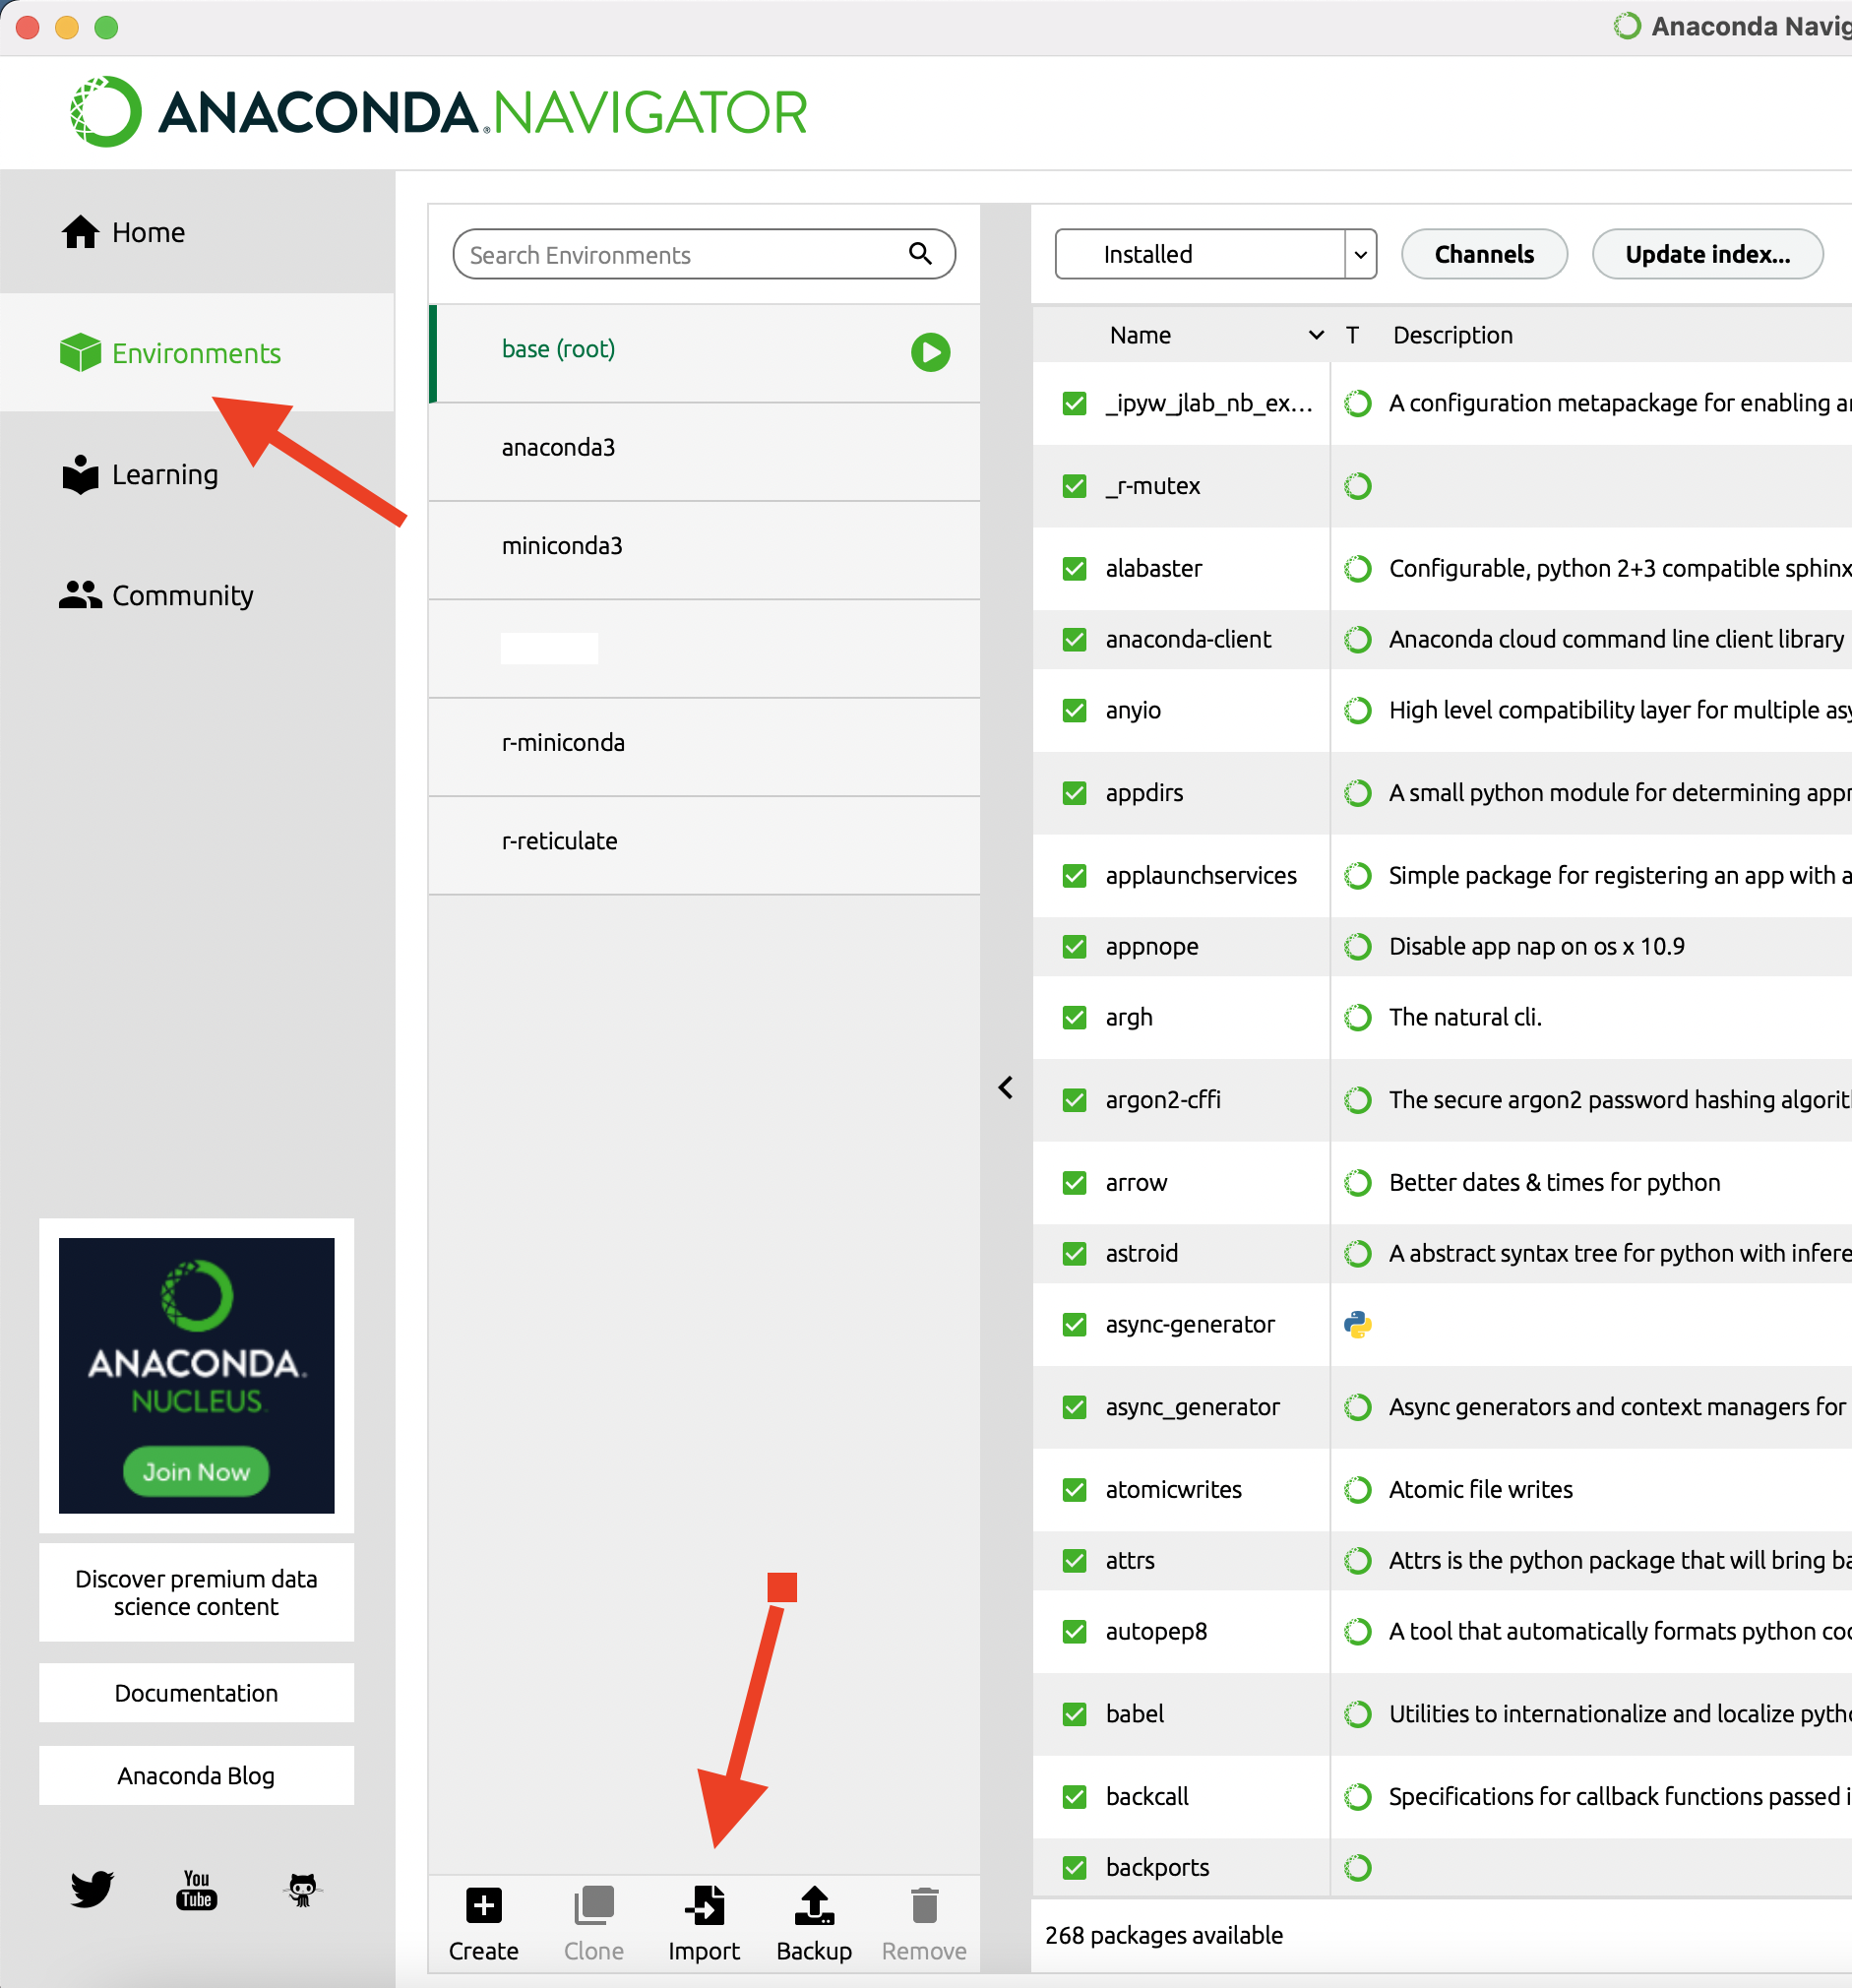
\includegraphics[scale = 0.20]{anaconda_navigator_1.png}
\end{frame}

\begin{frame}{WNE - Anaconda Navigator 2}
  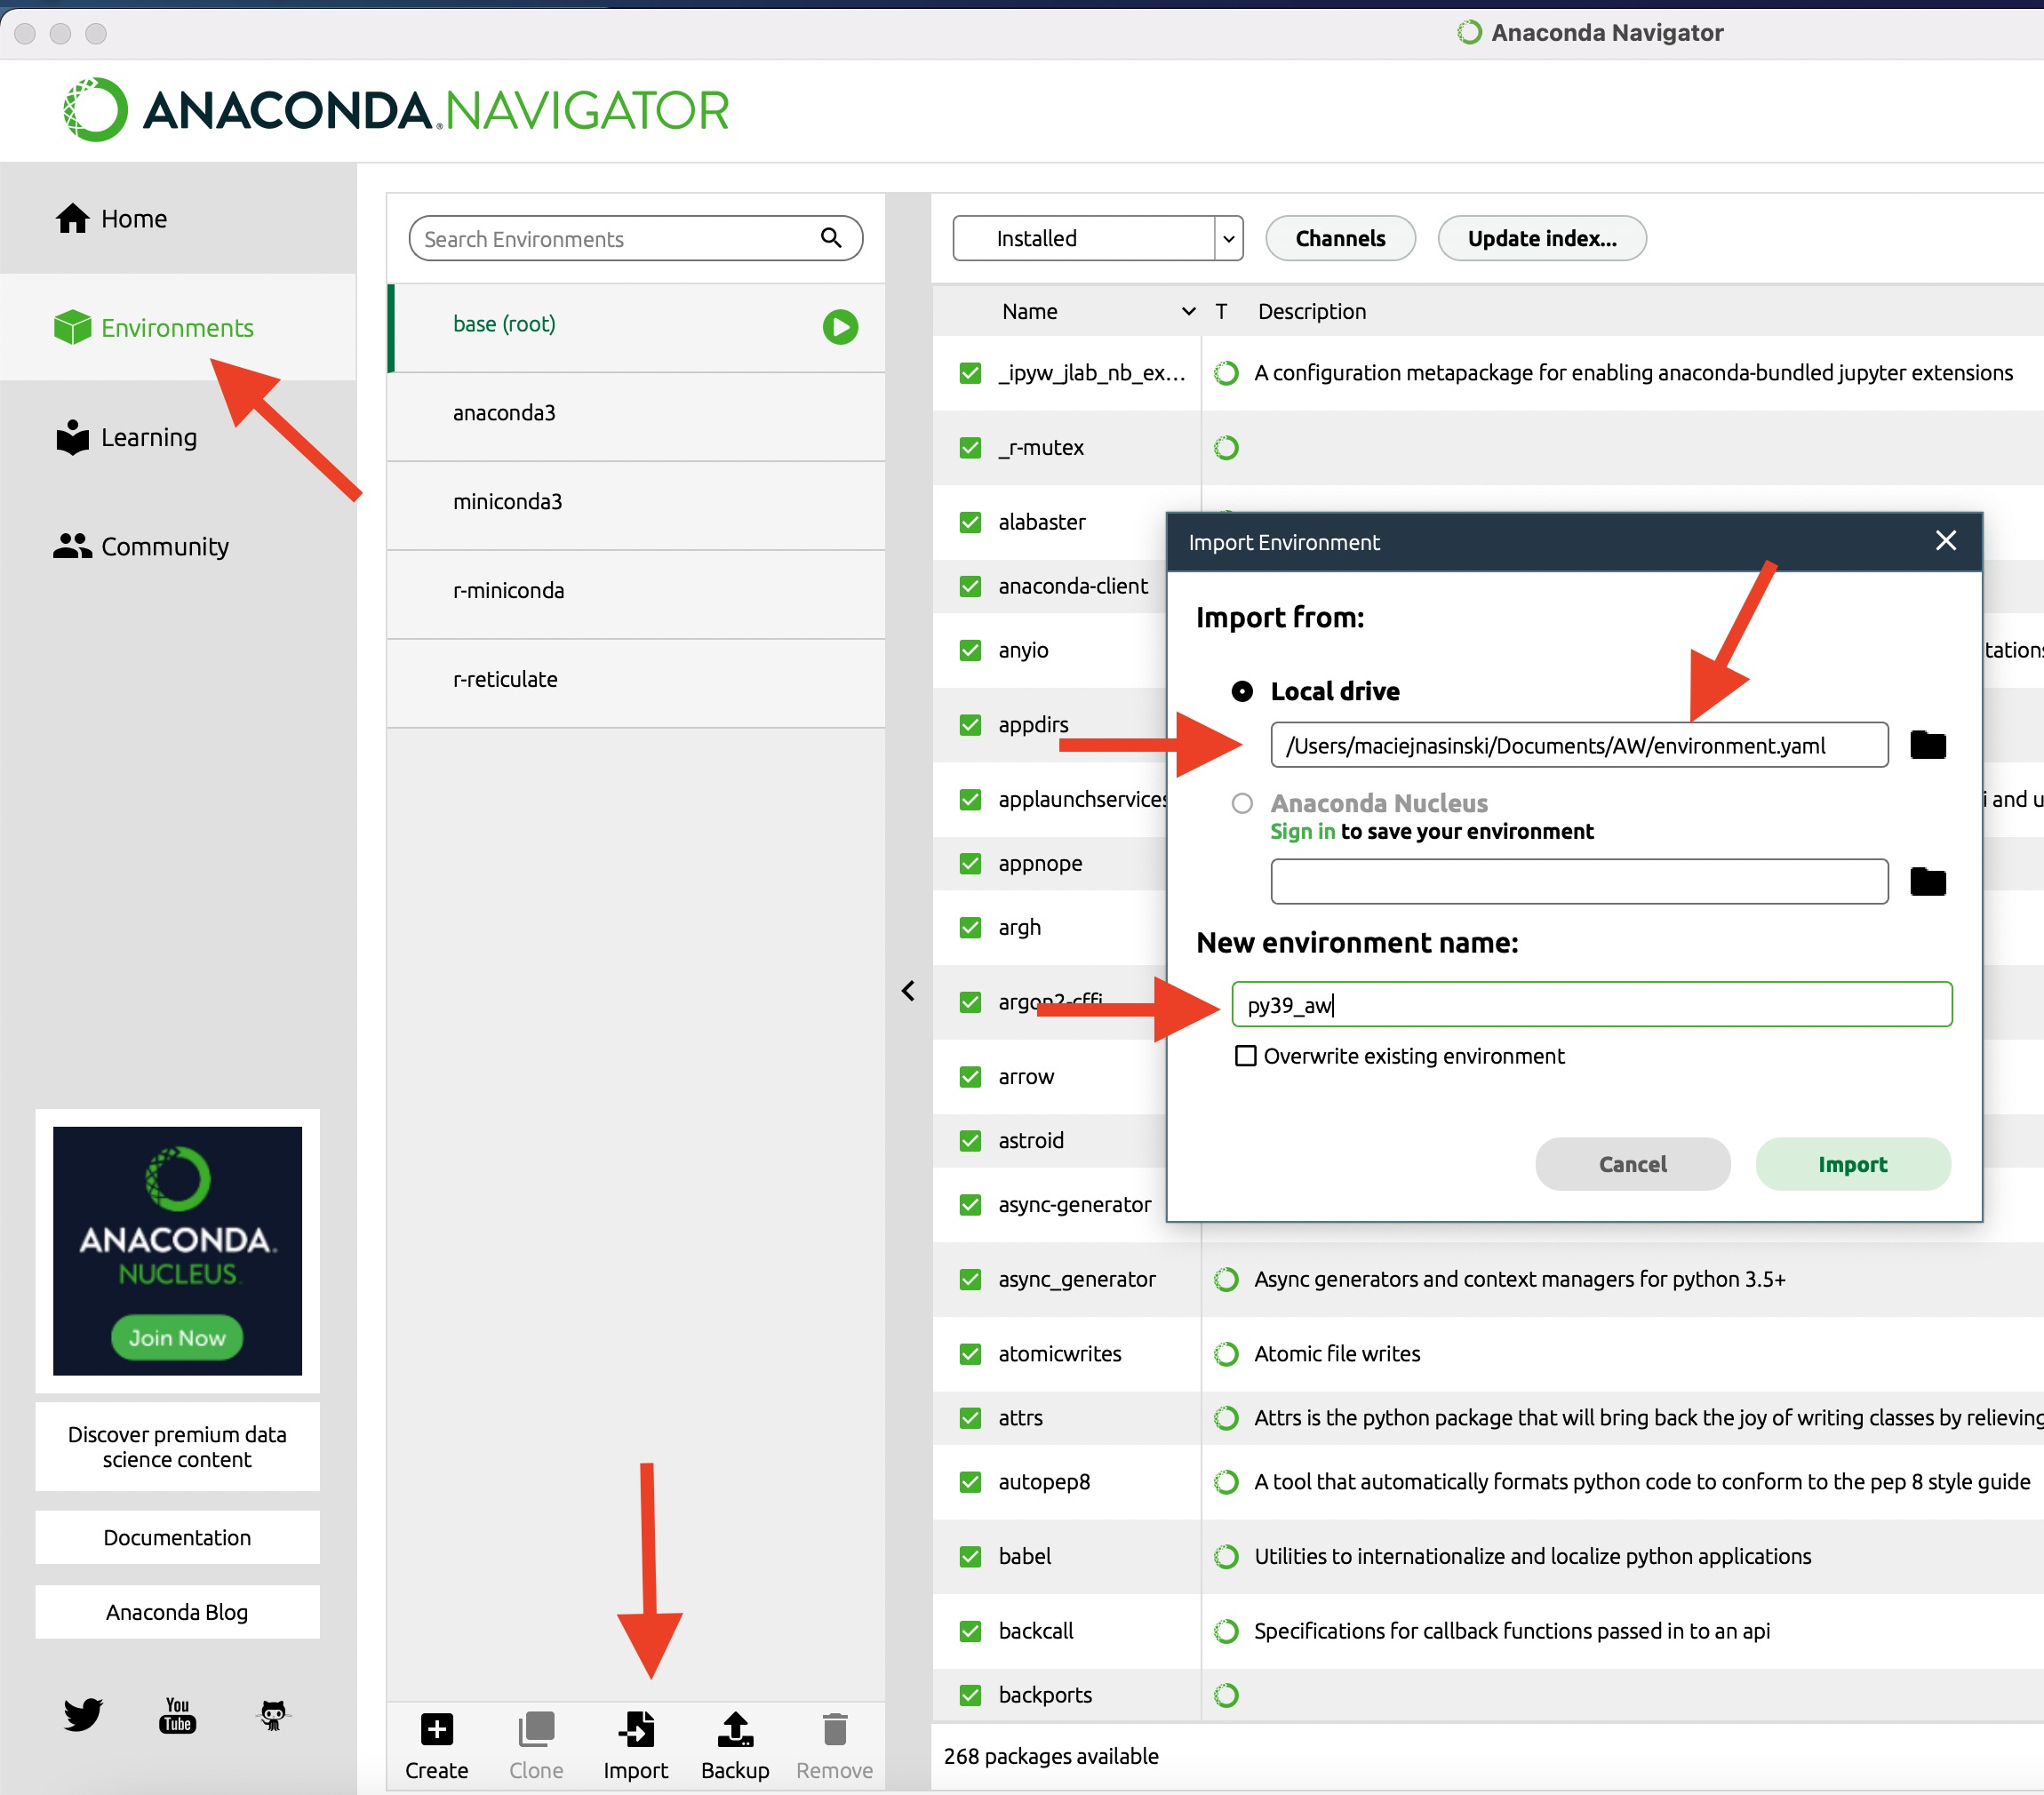
\includegraphics[scale = 0.20]{anaconda_navigator_2.png}
\end{frame}

\begin{frame}{WNE - Anaconda Navigator 3}
  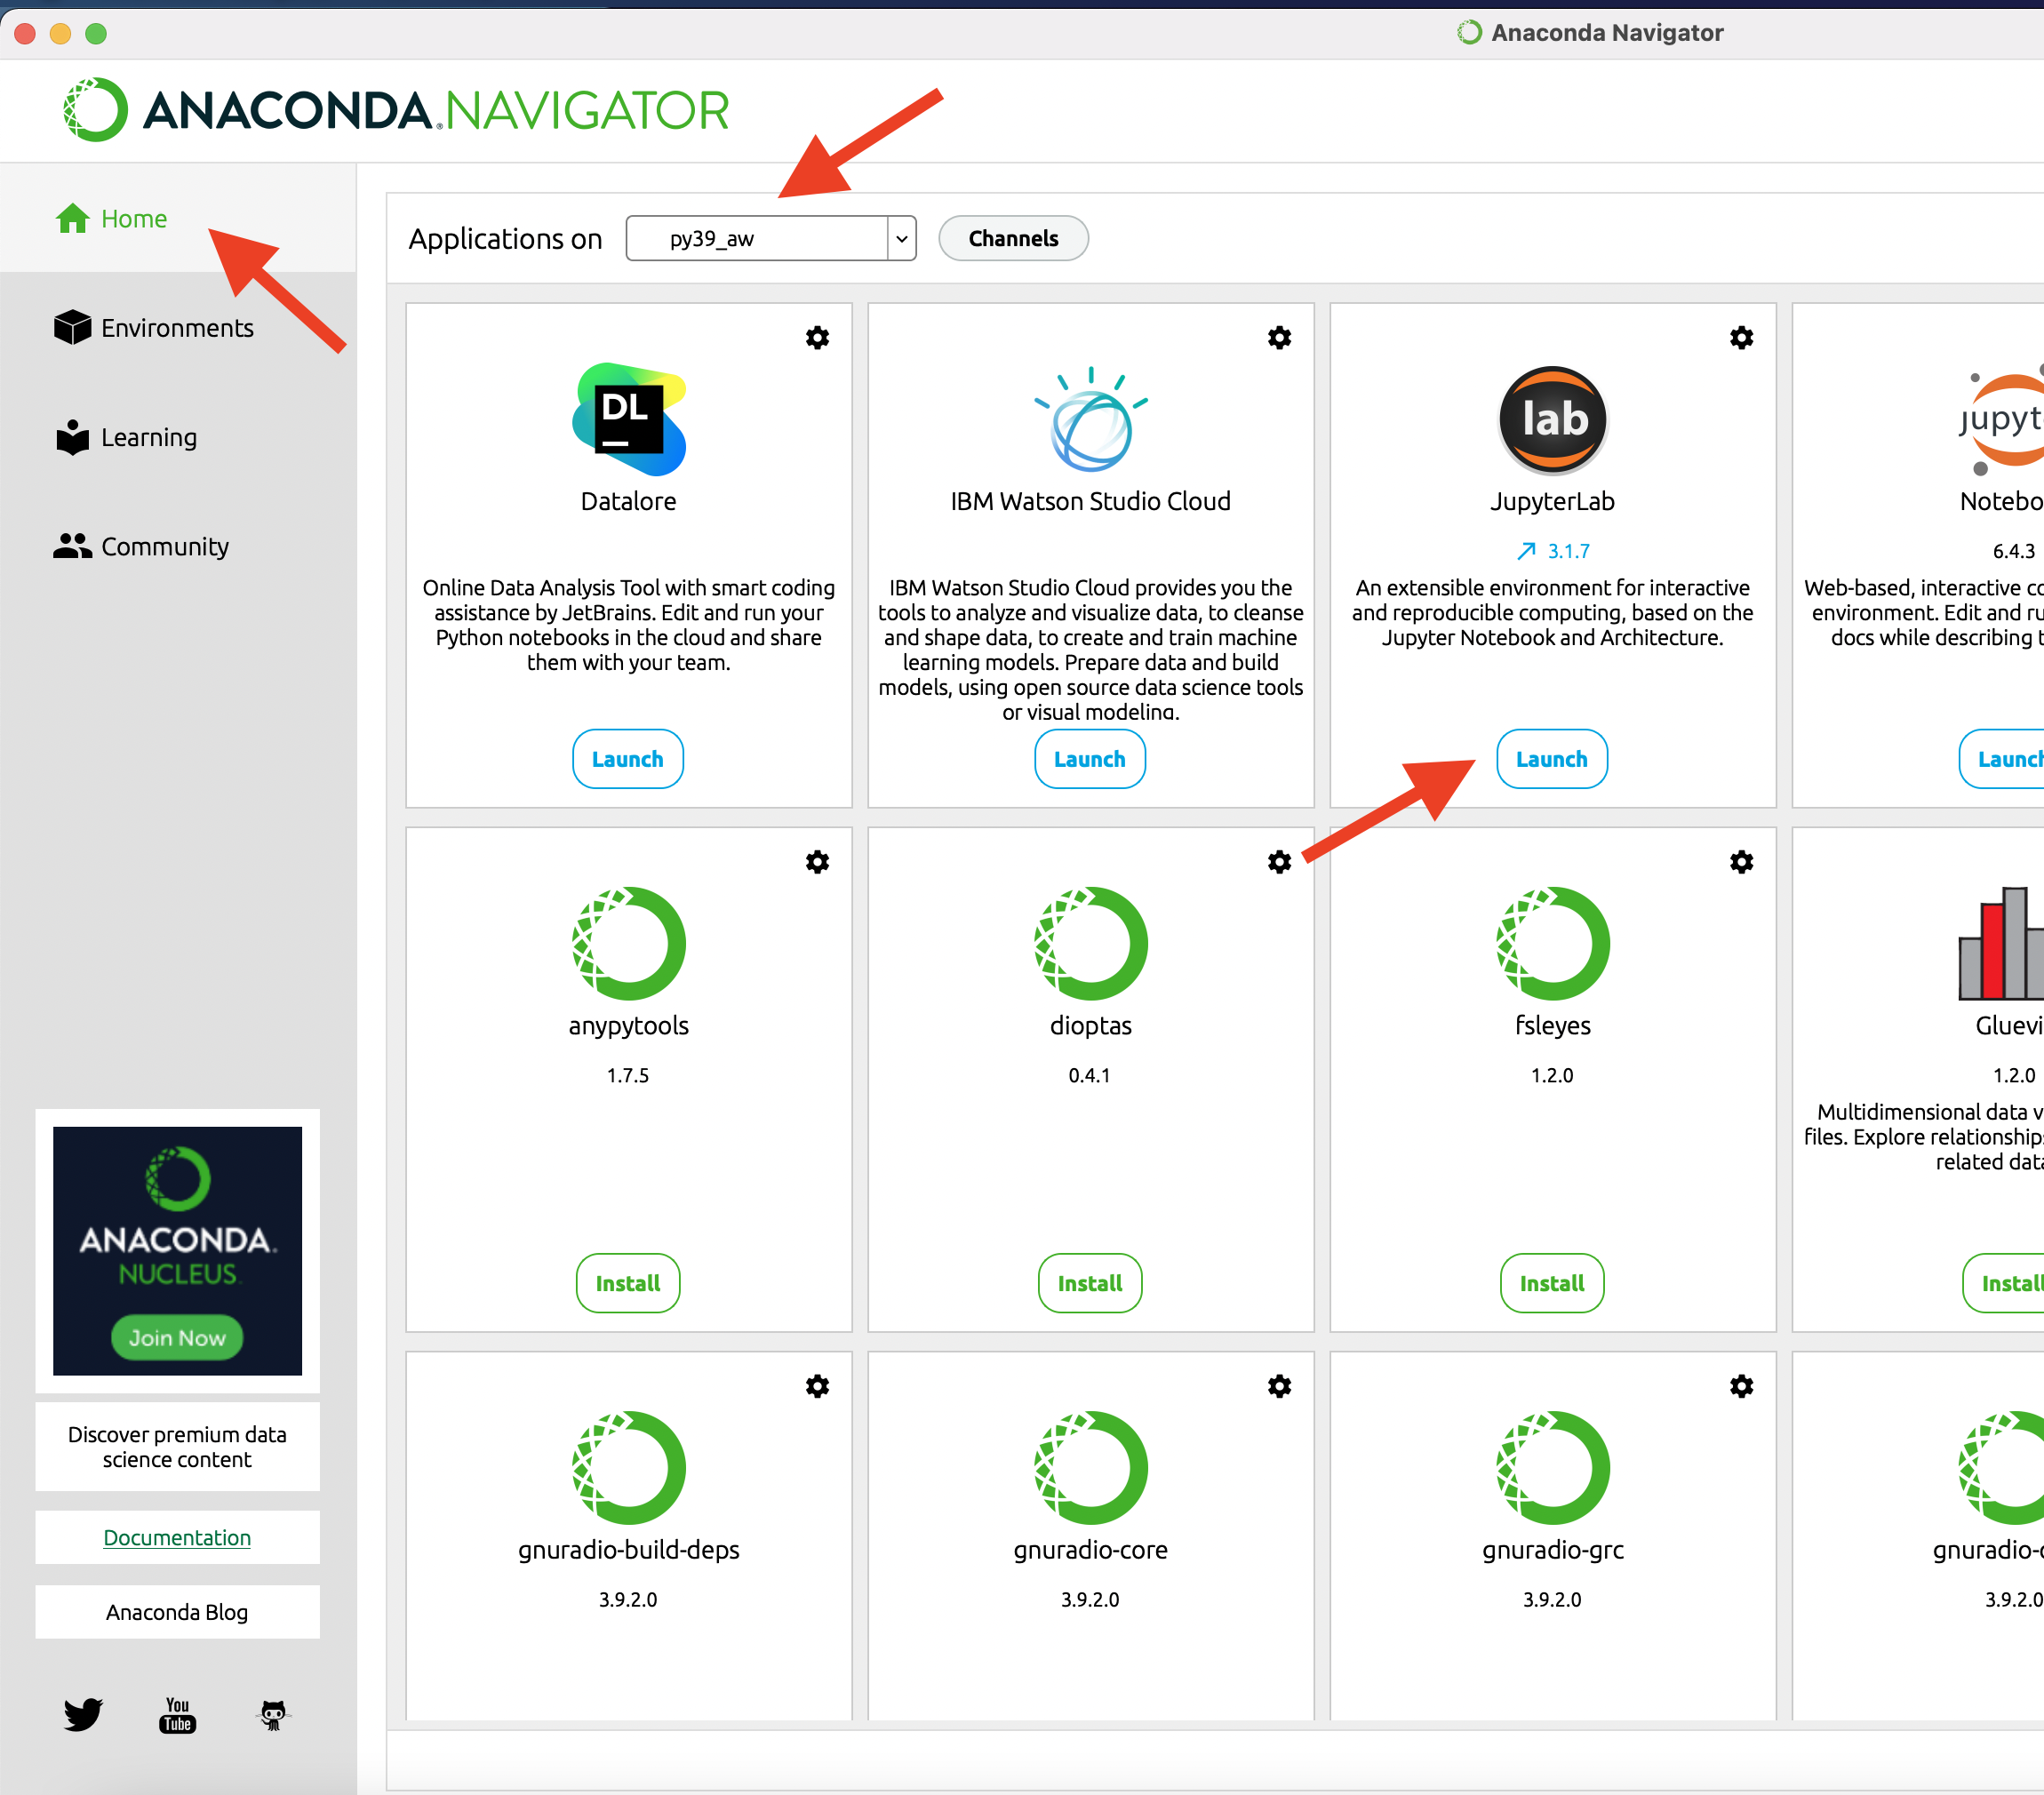
\includegraphics[scale = 0.20]{anaconda_navigator_3.png}
\end{frame}

\begin{frame}{Brak Anaconda}
  \item \texttt{pip3 install -r requirements.txt}
  \item \texttt{jupyter lab}
\end{frame}

\begin{frame}{Uaktualnienie Repozytorium AW2021}
  \item \texttt{cd AW2021} zmiana ścieżki na AW2021
  \item \texttt{MOZE BYC POTRZEBNY - git stash lub git commit -am "opis"}
  \item \texttt{git pull}
\end{frame}

\begin{frame}{STATA i python}
  \begin{itemize}
  \item Dokumentacja pakietu pystata \url{https://www.stata.com/python/pystata/index.html}
  \item Nasz GUI jupyter \url{https://jupyter.org/} oraz użycie wraz ze STATA \url{https://www.stata.com/new-in-stata/jupyter-notebooks/}
  \end{itemize}
\end{frame}

\section{Dodatki}

\begin{frame}{Kto pyta, nie błądzi}
  \begin{itemize}
  \item Forum dla statystyków i programistów - stackoverflow i kategoria cross validated \url{https://stackoverflow.com/}
  \end{itemize}
\end{frame}

\begin{frame}{Python - źródła}
  \begin{itemize}
  \item Python for Everybody \url{https://py4e.pl/book.php} or Python Crash Course \url{https://github.com/ehmatthes/pcc_2e}
  \item Znana strona z materiałami o pythonie \url{https://realpython.com/}
  \end{itemize}
\end{frame}

\end{document}
